\chapter{The XP2SHG/SFG Technique in Action}\label{chap_setup}
\minitoc
%%%%%%%%%%%%%%%%%%%%%%%%%%%%%%%%%%%%%%%%%% Gear %%%%%%%%%%%%%%%%%%%%%%%%%%%%%%%%%%%%%%%%%%%%
\section{Equipment and Setup}
All the samples used in this work were graciously provided by Dr. Jorge Alejandro Reyes Esqueda and Dr. Alicia Oliver of the Instituto de F\'isica de la Universidad Nacional Aut\'onoma de M\'exico (IF-UNAM). His group has published several articles that involved nanoparticles identical to these. These studies range from determining the third-order response \cite{torres2008optical, rodriguez2009large}, nonlinear absorption \cite{fernandez2011nonlinear, reyes2009anisotropic}, and deformation characteristics \cite{silva2010high, rocha2011second} of various nanosystems.

The XP2SHG/SFG and laser setup used to do this experiment is located in the Femtosecond Spectroscopy Lab at the University of Texas at Austin. Dr. Michael Downer generously allowed me to spend some time in this lab in order to finish the experimental phase of this research. I have mentioned several articles published by his group that go into some detail about the exact setup being used for different experiments. See references \cite{figliozzi2005single}, \cite{wirth2008second}, \cite{PhysRevB.84.165316}, and \cite{figliozzi2007shg} for more information.

All of this experimental work was done with the help and guidance of Junwei Wei, one of Dr. Downer's Ph.D. students. He does not appear in any of the pictures, but he was always there.

%%%%%%%%%%%%%%%%%%%%%%%%%%%%%%%%%%%%%%%%% Samples %%%%%%%%%%%%%%%%%%%%%%%%%%%%%%%%%%%%%%%%%%%
\subsection{Nanoparticle Samples}

We analyzed a total of three samples during the course of this research -- one gold (Au), one ionic gold ($\text{Au}^{2+}$), and one silicon (Si) sample. Each of these are embedded in glass ($\text{SiO}_{2}$) substrates via ion implantation. The substrates are made from Suprasil 300, which is a high quality fused silica specially designed for these types of applications. The substrate for all samples is about 500 micrometers thick.

\subsubsection{Ion Implantation}
Ion implantation is a method used to forcefully introduce atoms into a matrix. Ions penetrate fully into the matrix rather than staying at the surface when implantation occurs at energies higher than a few keV. Spherical nanoparticles form inside the matrix after thermally treating the sample under specific atmospheric conditions in a process called annealing. The formation of nanoparticles can be verified directly with a transmission electron microscope, or indirectly via optical measurements. The optical dispersion and absorption will coincide with the specific absorption bands associated with the plasmon resonance for each kind of nanoparticle.

\subsubsection{Gold Nanoparticles}\label{chap_setup_gold}
The two gold samples are roughly 8 by 4\,mm and 8 by 8\,mm respectively for Au and Au$^{2+}$. They are both pinkish in color to the naked eye. The gold ions are implanted at 2 or 3\,MeV with a dose of $8\times10^{16}$ ions per $\text{cm}^{2}$, annealed in an oxidizing atmosphere at $1100^{\circ}\,\text{C}$ for one hour. Nanoparticle size is around 3\,nm. See figure \ref{fig_tem_gold_np} for a TEM scan of the Au sample.

\subsubsection{Silicon Nanoparticles}
The silicon sample is 8 by 4\,mm in area, and is grayish in color to the naked eye. The Si ions are implanted at 1.5\,MeV with an average dose of $2.5\times10^{17}$ ions per $\text{cm}^{2}$. Annealing is done in a reducing environment of 50\% $\text{H}_{2}$ and 50\% $\text{N}_{2}$ at $1100^{\circ}\,\text{C}$ for one hour. Nanoparticle size is around 20 - 25\,nm. See figure \ref{fig_tem_si_np} for a TEM scan of the sample.

\begin{figure}[h]
\centering
\subfloat[Au nanoparticles.\label{fig_tem_gold_np}]{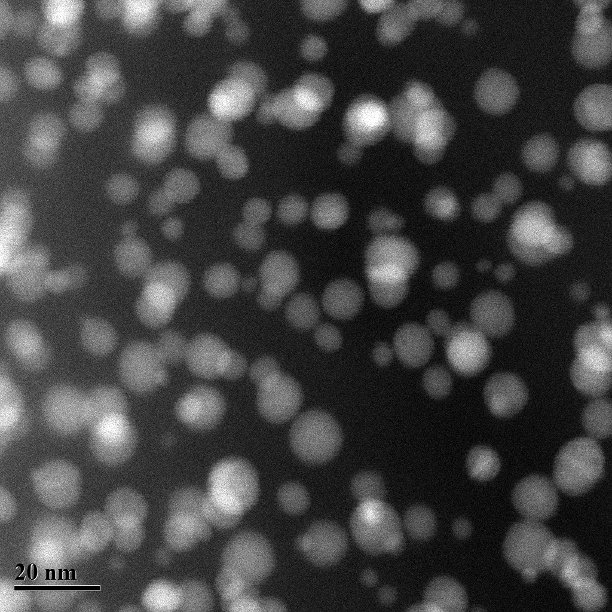
\includegraphics[width=0.5\textwidth]{setup/Au_8008}}
\subfloat[Si nanoparticles.\label{fig_tem_si_np}]{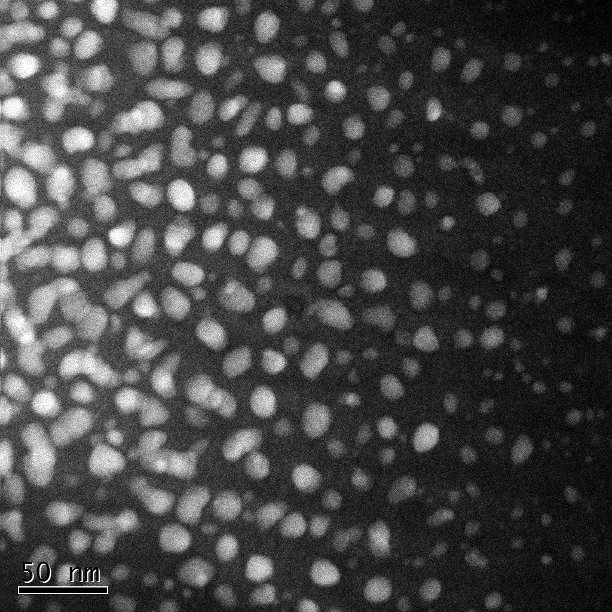
\includegraphics[width=0.5\textwidth]{setup/Si_front_0368}}
\caption{TEM scans for two of the samples.}
\end{figure}

\subsubsection{Reference Glass and Substrate}\label{chap_setup_glass}
In addition to the nanoparticle samples, a piece of the same substrate (Suprasil 300) used to embed the nanoparticles was included as a first reference. A second sample of high quality glass from the Femtosecond Spectroscopy lab was used as a second reference.

%%%%%%%%%%%%%%%%%%%%%%%%%%%%%%%%%%%%%%%%% Lasers %%%%%%%%%%%%%%%%%%%%%%%%%%%%%%%%%%%%%%%%%%%
\subsection{Laser System}\label{chap_setup_laser}
The laser used in this setup is a modular ultrafast system with a fundamental wavelength of 800\,nm. It consists of a Spectra-Physics Spitfire Ti:sapphire amplifier, coupled to a Spectra-Physics Merlin pump laser, and a KMLabs oscillator. Pumping the oscillator is a Spectra-Physics Millenia V. The pump and Ti:sapphire cooling is done via two stationary water chillers. Figure \ref{fig_lasers} is a photograph of the system.

The very large size of the amplifier and oscillator allows for easy modification and adjustment. As with most laser systems, we checked power output on a daily basis and  made the appropriate adjustments to maximize available power.

\begin{figure}[h]
\centering
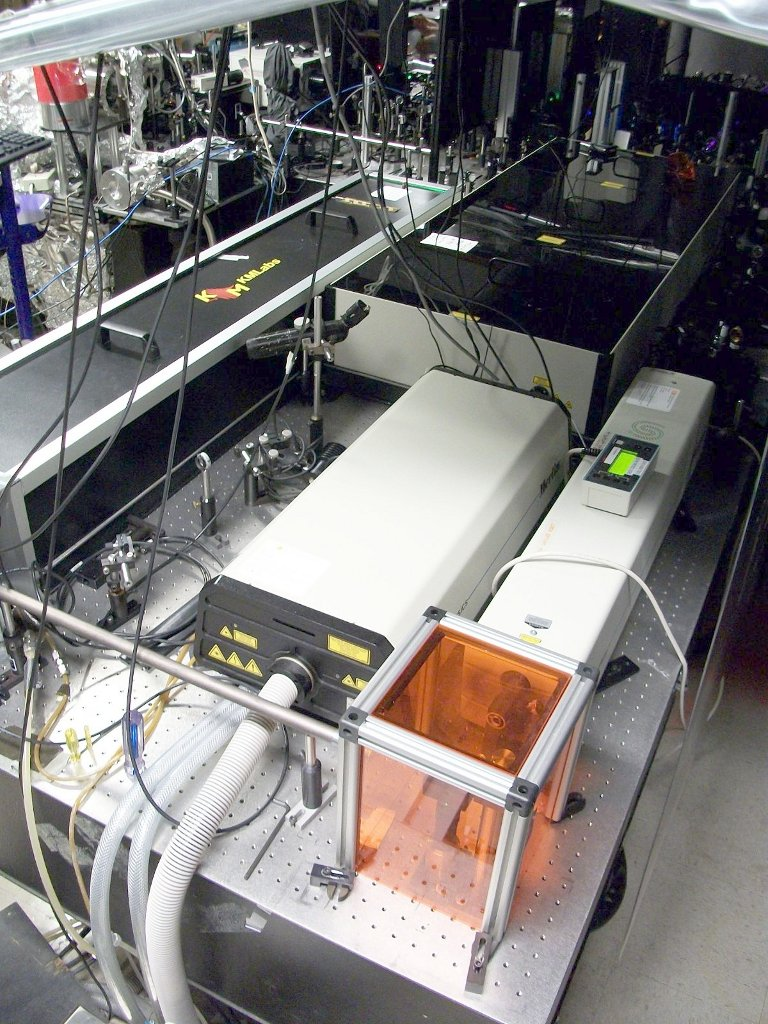
\includegraphics[scale=0.55]{setup/lasers}
\caption[Laser system used in experiment.]{Laser system used in experiment. Clockwise from right: Millenia V, Merlin, KMLabs oscillator, and Spitfire in back.\label{fig_lasers}}
\end{figure}

\subsubsection{Spectra-Physics Millenia V Pump Laser}
This laser pumps the oscillator. It is a diode-pumped, continuous wave, solid-state visible laser that outputs 4.30\,Watts at 532\,nm. It uses a neodymium yttrium vanadate (Nd:YV$\text{O}_{4}$) gain medium that is pumped by two 20\,Watt fiber coupled diode laser bars that are located in the control box. The Nd:YV$\text{O}_{4}$ crystal produces 10\,Watts power at 1064\,nm after amplification. The light is then doubled with a lithium triborate (LBO) crystal to produce close to 5\,Watts.

\subsubsection{KMLabs Ti:sapphire Laser Kit}
The oscillator system is a KMLabs Ti:sapphire Laser Kit. It was designed to be built and alligned by the user and was sold disassembled. It requires close to 4.5\,Watts of 532\,nm pump light in $\text{TEM}_{00}$ mode to produce a 10 - 15\,fs pulse with a bandwidth of 50 - 70\,nm FWHM and an average power of 500\,mW. It has a repetition rate of 76\,MHz. This laser was by far the best behaved during the course of this experiment. Although it needs to be constantly realigned to maximize output, it never stopped working.

\subsubsection{Spectra-Physics Merlin Pump Laser}
This laser acts as the pump for the amplifier. It is a 527\,nm Q-switched pump laser that uses a neodymium-doped yttrium lithium fluoride (Nd:YLF) active medium. The Nd:YLF rod is optically pumped with an arc lamp and is water cooled. The rod emits light at 1053\,nm, which is then doubled by an LBO crystal to 527\,nm. It has a repetition rate of 1\,kHz and produces 10\,mJ of energy per pulse. 

\subsubsection{Spectra-Physics Spitfire Laser Amplifier}
The Spitfire is a regenerative Ti:sapphire amplifier. It uses two gratings for stretching and compressing the pulse, as is normal with CPA systems. The final output is 1.1 Watts with 1 mJ per pulse at 800\,nm with a pulse duration of around 100\,fs.

%%%%%%%%%%%%%%%%%%%%%%%%%%%%%%%%%%%%% NOPA %%%%%%%%%%%%%%%%%%%%%%%%%%%%%%%%%%%%%%%%%%%%%%%%%
\subsection{NOPA at Femtosecond Spectroscopy Lab}

We learned about the concepts behind the NOPA in section \ref{chap_theory_nopa}. This NOPA uses a beta barium borate (BBO) crystals to produce SHG. A sapphire window generates the white light continuum needed to seed the crystal. All the elements in the beam path stretch the pulse temporally -- two large prisms are used to re-compress it back down to an acceptable length.

It is tunable via a delay stage. However, it is not a straightforward matter of adjusting the stage and getting a new wavelength. Some parts of the system need to be realigned after moving the stage even a little.

This NOPA produces pulses that are around 250\,fs in duration with a 1\,kHz repetition rate. Pulse energy is between 3 - 12\,$\mu$J, and can be tuned between 1.6 and 2.4\,eV, or 760 - 515\,nm. Figure \ref{fig_nopa_diagram} depicts a diagram of the setup, while figure \ref{fig_nopa_work} shows the NOPA in action.

\begin{figure}[h]
\centering
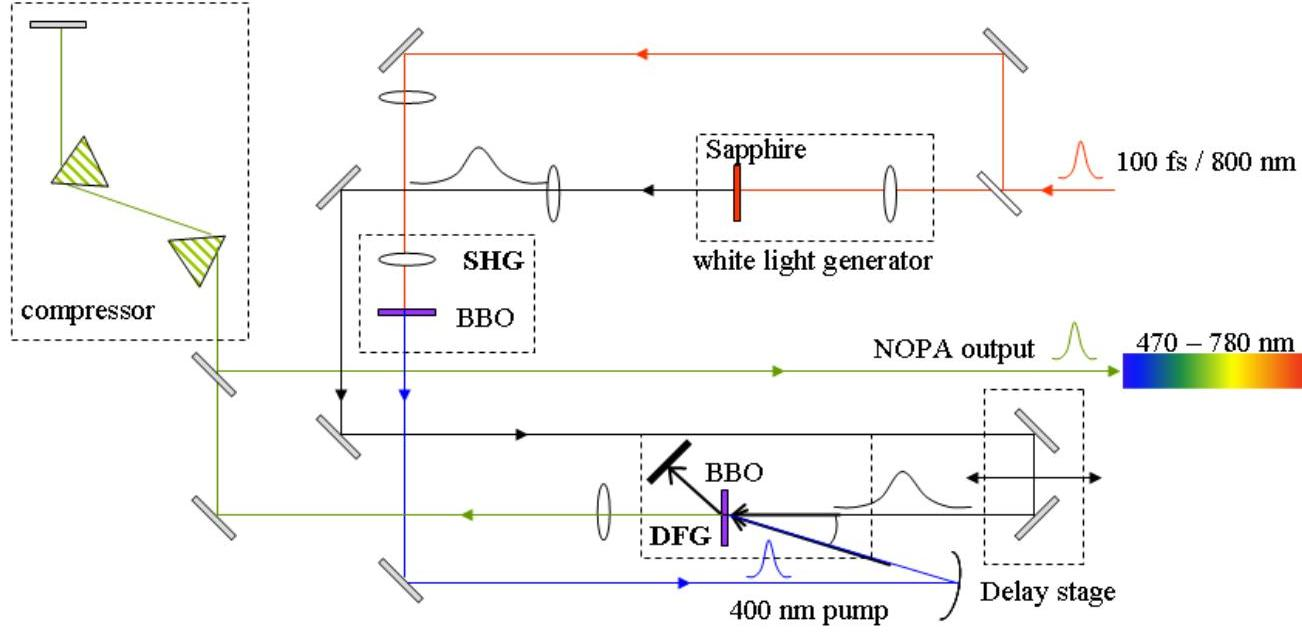
\includegraphics[width=0.95\textwidth]{setup/nopa}
\caption[Diagram of the NOPA at the Femtosecond Spectroscopy Lab.]{Diagram of the NOPA at the Femtosecond Spectroscopy Lab. Image: Adrian Wirth, Junwei Wei.\label{fig_nopa_diagram}}
\end{figure}

\begin{figure}[h]
\centering
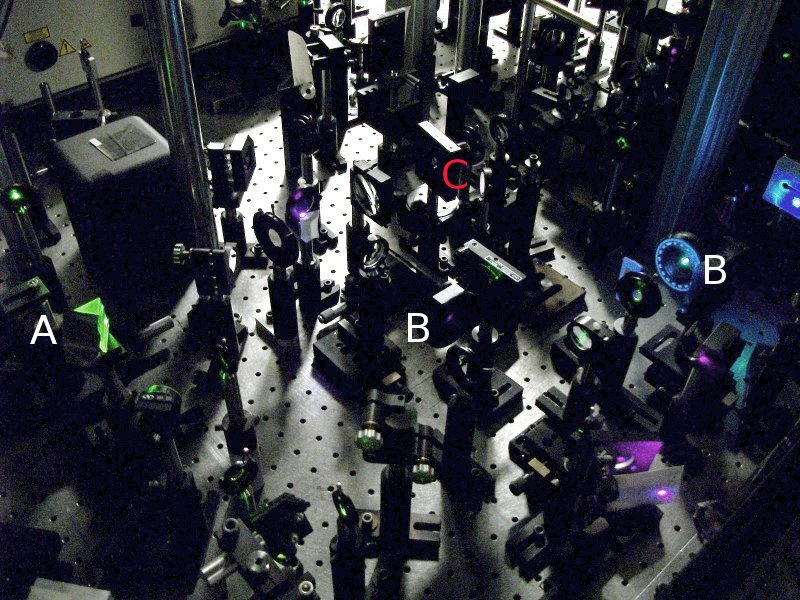
\includegraphics[width=0.95\textwidth]{setup/nopa_pic}
\caption[The NOPA at the Femtosecond Spectroscopy Lab.]{The NOPA at the Femtosecond Spectroscopy Lab. One prism (A), two crystals (B), and the sapphire window (C) can be seen.\label{fig_nopa_work}}
\end{figure}

%%%%%%%%%%%%%%%%%%%%%%%%%%%%%%%%%%%%%% XP2SHG/SFG %%%%%%%%%%%%%%%%%%%%%%%%%%%%%%%%%%%%%%%%%%%
\subsection{The XP2SHG/SFG Elements}
We discussed the foundations for this technique in section \ref{chap_theory_xp2}. The arrangements for both SHG and SFG are very similar; amplified pulses from the laser are used for SHG, and the off-normal beam with the NOPA output is used for SFG. Physically, the setup is a modular optical arrangement placed on two breadboards that snap into place with strong magnets. This allows for easy removal and fast adjustments. Different arrangements can be put in place without totally misaligning the entire setup. The first breadboard contains the delay stage, beam-splitter, and mirrors that allow for fine adjustments and provide the reference signal for the experiment.

\subsubsection{XP2SHG Arrangement}
I will describe the arrangement making reference to the diagram in figure \ref{fig_xp2}. The laser beam is first polarized via a thin film plate polarizer (not pictured), which ensures that the beam is p-polarized. It is then split by a piece of microscope slide (BS1) -- the weak reflection is focused down into a BBO crystal to produce second harmonic light at 400,nm, and is collected by an Oriel spectrometer to use as a quadratic reference.

The main beam is split by a 50/50 beam-splitter (BS2). The straight beam goes into a 1 cm delay stage used as a variable time delay in order to temporally overlap the pulses on the sample. This beam arrives at the sample at normal incidence, so dipolar SHG from the substrate surface is strictly forbidden by selection rules. Lastly, it is focused down via a fixed 50\,mm lens (L3).

The other beam is redirected through a half-wave plate (WP) which polarizes it vertically. It arrives at the sample s-polarized, and initially at an angle $\phi_{0}$ of 20 degrees. Later on we separated the beams further to avoid scattering and increased the angle to 40 degrees. Dipolar SHG is also forbidden from the substrate surface for this beam as long as it is s-polarized. This beam is focused with a 50\,mm lens (L4). There is an optional BBO crystal on a folding arm that can be used to verify spatial and temporal overlapping of the two beams. This crystal cannot be used once the sample is in place. Figure \ref{fig_xp2_assembly} shows the second breadboard containing these elements. Figure \ref{xp2shgdark} depicts how intense the SHG signal is when everything is overlapped properly using the BBO crystal.

\begin{figure}[h]
\centering
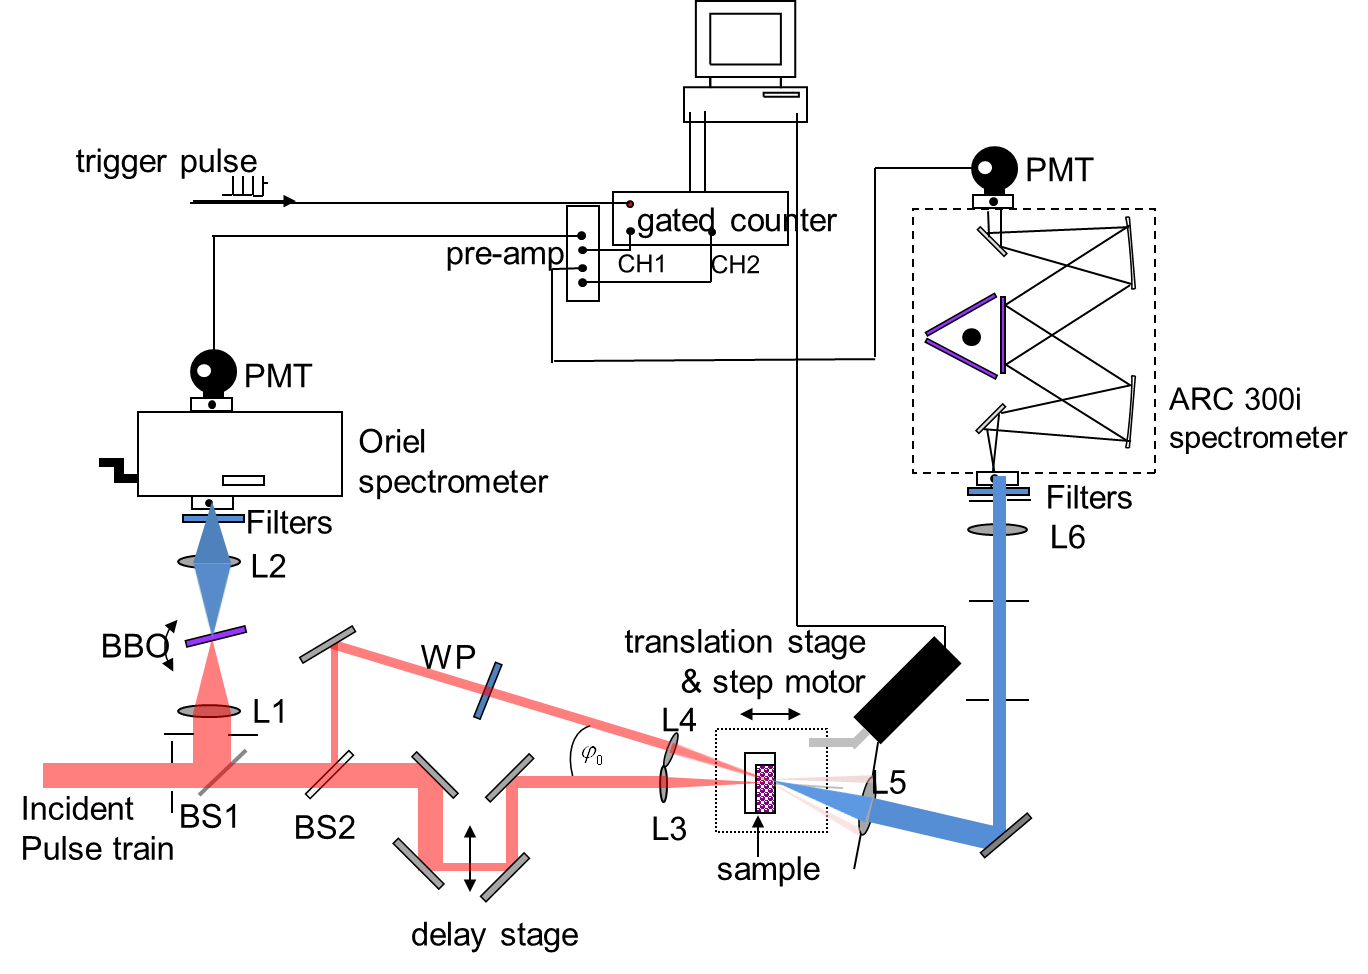
\includegraphics[width=\textwidth]{setup/XP2SHG_setup}
\caption[A diagram of the XP2SHG arrangement.]{A diagram of the XP2SHG arrangement. Image: Junwei Wei.\label{fig_xp2}}
\end{figure}

Finally, the beams are focused down on the sample with an approximate spot size of 250\,$\mu$m. Behind the sample is an iris with a collecting lens (L5). From there, the signal is captured by the ARC 300i monochromator/spectrometer. I will describe these detectors in greater length in section \ref{chap_setup_det}.

The sample holder is built on a linear translation stage. It is controlled by a stepper motor that can be accessed via a computer. This allows us to control the motion of the sample during the experiment; the motion is stopped automatically with the recording of each data point.

\begin{figure}[h]
\centering
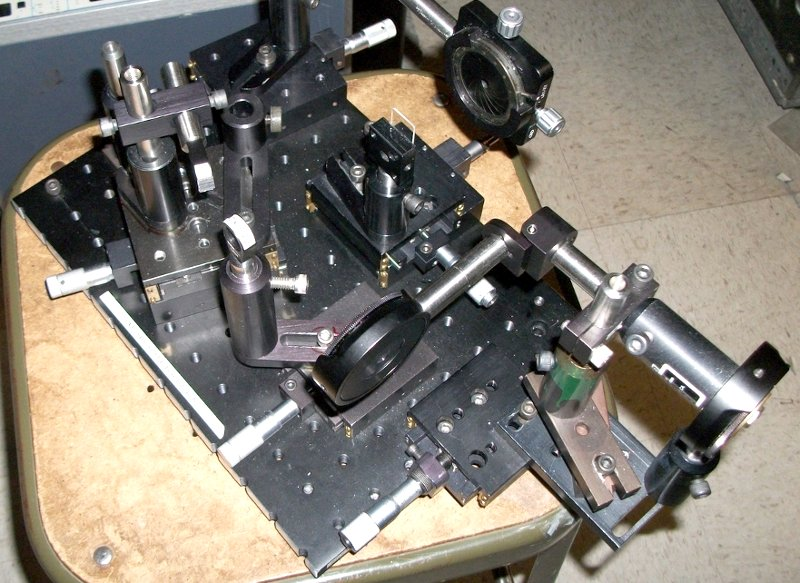
\includegraphics[width=0.86\textwidth]{setup/xp2shg_assembly}
\caption[Second XP2SHG breadboard.]{Second XP2SHG breadboard. Substrate sample in holder and BBO crystal folded away at middle.\label{fig_xp2_assembly}}
\end{figure}

\begin{figure}[h]
\centering
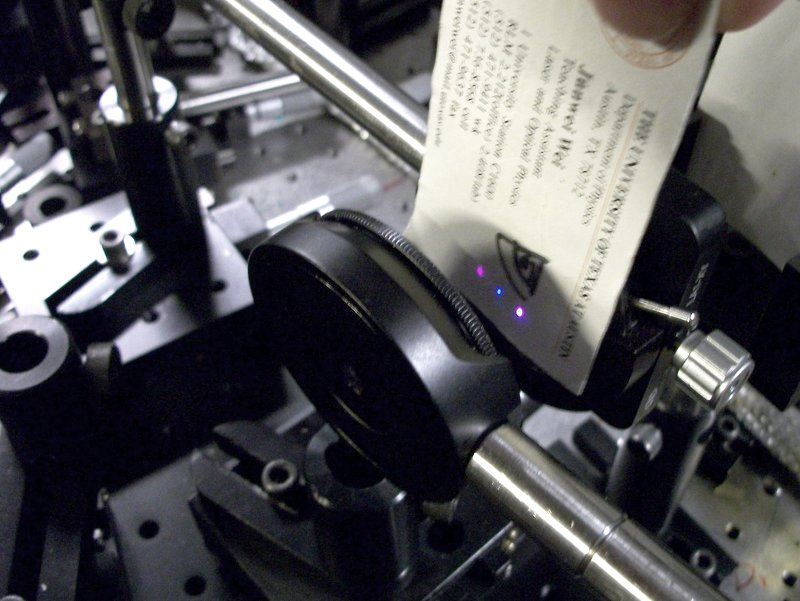
\includegraphics[width=0.86\textwidth]{setup/xp2shgdark}
\caption{XP2SHG with a BBO crystal.\label{xp2shgdark}}
\end{figure}

\subsubsection{XP2SFG Arrangement}
The arrangement remains very similar for SFG measurements. First, we get the NOPA up and running. After it is functioning at maximum efficiency, its output is fed into the XP2SFG path. BS2 is no longer needed, but the output is typically so energetic that it is easier to leave it in and block the redirected beam. In its place, a beam split off from the main amplifier output is used. This beam comes around the entire setup and an extra mirror must be inserted to redirect the new beam into the focusing lens. When set up like this, we used two filter holders (one for each beam) to provide fine attenuation to each. These consisted of various neutral density and color filters (UG5 and OG515).

%%%%%%%%%%%%%%%%%%%%%%%%%%%%%%%%%%%%%%% Detectors %%%%%%%%%%%%%%%%%%%%%%%%%%%%%%%%%%%%%%%%%%
\subsection{Detection System}\label{chap_setup_det}
The detection system captures two sources of light -- the light produced from the sample, and a reference beam that we use to compare with the sample signal. Having the reference is important to correlate fluctuations in the laser output with corresponding fluctuations in the signal output. After we get the data we can normalize the signal data with the reference data to get a more accurate idea of what happened during the run.

The signal beam is captured in a Acton Research Corporation SpectraPro-300i monochromator, with a Hamamatsu R4220 photomultiplier tube (PMT) attached to it (figure \ref{fig_monochromator}). The ARC SpectraPro-300i is a 30\,cm monochromator that allows three grating choices. It is attached to a computer system with proprietary software installed that allows for manual grating and wavelength selection, or automated scans across a range.

The reference beam is captured by an Oriel 77250 monochromator coupled to another Hamamatsu R4220 PMT. The Oriel 77250 is a 12.5\,cm, single grating monochromator that is manually controlled via a hand-crank to turn the grating. It has no software control.

An Ocean Optics fiber spectrometer is sometimes used to determine the wavelength of the signal beam in the NOPA. It is PCI format and located inside a computer. A fiber is connected to it with the other end placed in the optical setup when needed. It is not used for recording data.

\subsubsection{Hamamatsu R4220 PMT}
The Hamamatsu R4220 PMT is a side-on, 28\,mm PMT. It detects in the range of 185 - 710\,nm, with its peak sensitivity at 410\,nm and a quantum efficiency of around 22\% at that wavelength. Although it has a broad sensitivity curve, it has the highest sensitivity and quantum efficiency in the 300 - 450\,nm range. This makes it optimal for detecting SFG and SHG signals which usually are between 300 - 400\,nm. The cut off wavelength is around 750\,nm, so it does not detect the Ti:sapphire fundamental of 800\,nm. It has a built in high voltage power supply that requires 15\,V to function. 

\begin{figure}[h]
\centering
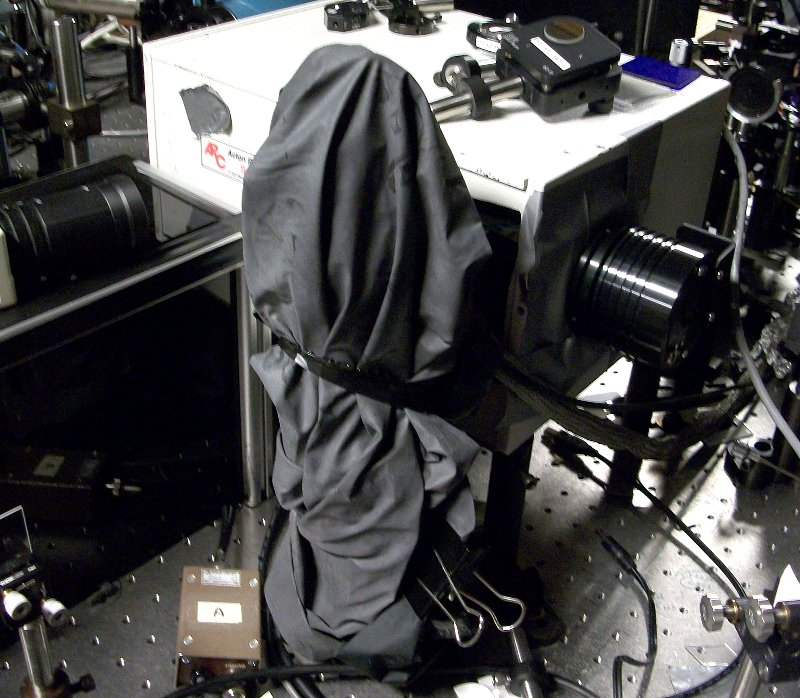
\includegraphics[width=0.9\textwidth]{setup/monochromator}
\caption{ARC SpectraPro-300i Monochromator with shrouded PMT.\label{fig_monochromator}}
\end{figure}

\subsubsection{Electronics}
Several pieces of electronic equipment are needed to control and record the signals from the PMTs. The measurement equipment is primarily manufactured by Stanford Research and is mounted in an Ortec 401A Modular System Bin. Outside of the bin reside the power supply for the PMTs, the Stanford Research SR400 photon counter, a Tektronix 7903 oscilloscope, and the computer used to control and record all data runs. See figure \ref{fig_electronics} for a picture of the setup.

\subsubsection{Equipment in Ortec 401A}
Inside the Ortec 401A is all Stanford Research equipment. The SR240 Fast Preamp is the amplifier used for both PMTs. Each PMT signal gets amplified two times in the SR240. The output of a PMT is connected to the input of one channel, then its output gets connected to the input of a second channel. The final output of each goes either to the SR250 gated integrator, or to the SR400 photon counter. The SR240 is a 350 MHz preamplifier with a gain factor of 5 per channel; this means that the output of each PMT is increased 25 times.

The SR245 is a computer interface that has both serial and GPIB ports to communicate with computers. This module is not in use however, since the computer system has its own PCI GPIB card.

Lastly, the SR250 Gated Integrator. This boxcar integrator is designed for signal recovery and is especially suited for use with fast events. It consists of a gate circuit that is only activated when externally triggered. In this way, the integrator is very useful for signal recovery because integrates and averages during very small windows of time. If the noise floor is relatively high, this can effectively isolate a signal and recover its features over the course of the measurement. The external trigger in our setup is supplied by the laser amplifier. However, since this device integrates and averages, it is no good for extremely small signals like the ones emitted by the samples which would get lost when averaged together. So this device is only used when optimizing and calibrating the setup.

\subsubsection{Stanford Research SR400 Photon Counter}
The SR400 is a dual channel photon counter that offers very sensitive, single photon measurements. It integrates amplifiers, discriminators, gate generators, and counters all in one unit. Each channel has its own set of instrumentation and can count at rates up to 200 MHz. Discriminators allow individual pulses to be filtered out from background noise. 

This piece of equipment was the cornerstone of this entire experiment. Our SHG and SFG signal strength was in the hundreds of photons (per two or three seconds) for our best runs. Only a photon counter, coupled with a very good PMT can read and record such low signals.

\begin{figure}[h]
\centering
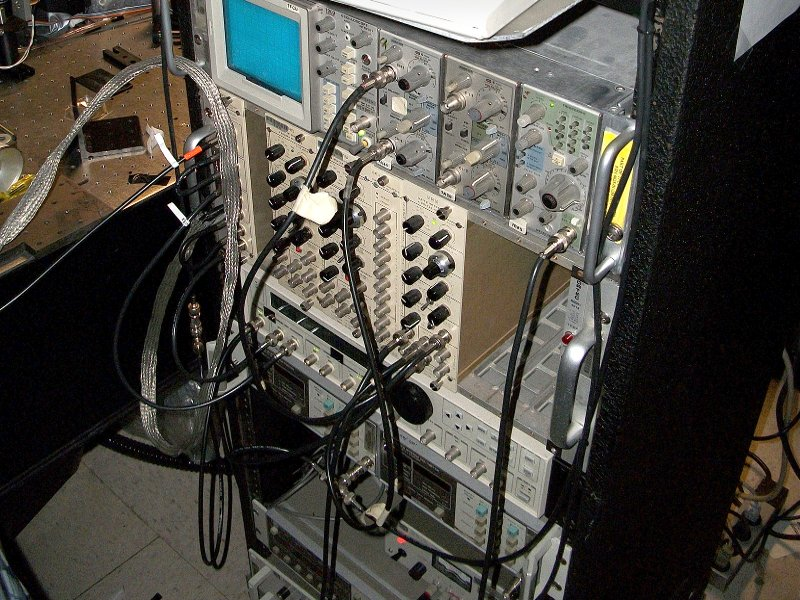
\includegraphics[width=0.9\textwidth]{setup/electronics}
\caption[Electronics for detection equipment.]{Electronics for detection equipment. From bottom device with red light: power supply for PMTs, HP Voltimeter, Stanford Research SR400, Ortec 401A, and Tektronix 7903 oscilloscope. In Ortec rack from left to right: SR240 Fast Preamp, 2 $\times$ SR250 Gated Integrator, SR245 Computer Interface, and SR250.\label{fig_electronics}}
\end{figure}

\subsubsection{Computer System}
The computer system is a standard desktop machine that runs homebrew NI LabVIEW programs under Microsoft Windows 2000. These programs control the movement of the sample holder which is located on a linear stage, and simultaneously record data at each stop. The program most used for this research records the stage position in steps, the SHG/SFG signal, the reference signal, and the ratio of the two. It has its own GPIB interface which is directly connected to the SR400 for data acquisition. This data is stored in a simple text file for later plotting and analysis.

%%%%%%%%%%%%%%%%%%%%%%%%%%%%%%%%%%%%%%%%%%%%%%%    %%%%%%%%%%%%%%%%%%%%%%%%%%%%%%%%%%%%%%%%%%%%%
%%%%%%%%%%%%%%%%%%%%%%%%%%%%%%%%%%%%%%%%%%%% Procedure %%%%%%%%%%%%%%%%%%%%%%%%%%%%%%%%%%%%%%%%%
\section{Procedure}
\subsection{Linear Measurements}
The linear measurements for the samples were taken at the Center for Nano and Molecular Science and Technology in the Nano Fabrication and Testing Facility at UT Austin. The samples underwent linear transmittance analysis in a Varian Cary 500 UV-Vis Spectrometer, and spectroscopic ellipsometry (SE) in the cleanroom using a J.A. Wollam M2000 Spectroscopic Ellipsometer. Thanks go to Junwei Wei for taking these measurements.

\subsection{Adjustments Prior to Running XP2SHG/SFG}

\subsubsection{Optimizing Laser Output}
The first step for the XP2SHG experiment is optimizing the laser output into the optical arrangement. We turn the laser system on and  leave it running for about half an hour to ensure stability. Then, the laser power is measured at the exit aperture using a power meter. The delay times for the Pockels cells are adjusted for maximum output using the same power meter. A mirror is placed in front of the Spitfire output beam reflecting it through a lens that focuses the beam down. A screen shows the resulting nonlinear blotch produced by the plasma being created by the beam. Adjusting the compressor length inside the Spitfire via the motorized adjustment control changes the brightness and color of the blotch; the output of the laser is at its most energetic when at maximum brightness.

\subsubsection{Optimizing Overlaps and SHG/SFG Output}
The signal from the laser or the NOPA arrangement (for SHG or SFG) is introduced into the XP2SHG/SFG optics after the laser system has been set to maximum output. However, a good stable laser signal is not enough to ensure that the XP2SHG setup will work correctly -both beams need to be both spatially and temporally overlapped.

Spatial overlap is usually done by eye. The two beams are placed on a screen located at the focal point of the two lenses and the mirrors are adjusted until both hit the same spot on the screen. This can be verified using a telescope lens arrangement, but this method is rarely used as visual confirmation is good enough. Regardless of SHG or SFG, the two beams must coincide as closely as possible. A business card works as a screen although the NOPA beam in SFG is usually dimmed because the human eye is extremely senstive to green and it appears to overpower the 800 nm beam.

The BBO crystal is then swung into place above the sample holder. It is designed to be at the common focal point of both lenses. Its mount can be rotated to facilitate proper phase-matching conditions. Only proper spatial and temporal overlapping will allow the crystal to produce the SHG/SFG signal. The direction of the output signal is always exactly between the other two beams. See figure \ref{xp2shgdark} for a picture of the BBO output.

At last we come to the question of finding the temporal overlap. Both of the beams consist of trains of pulses that move along the optical path. Pulses from both trains have to coincide at the same time on the sample in order to produce a nonlinear signal. This is adjusted via the delay stage for the normal incidence beam and has to be done if any adjustment is made to the setup that changes the optical path. This includes the introduction of filters or moving any element along the beam line. Once a position is set on the micrometer adjuster, it can typically be referred back to as long as the path has not changed.

In summary, a normal overlap adjustment consists of simultaneously adjusting off beam mirror, the rotation on the crystal, and the delay stage on the beam at normal incidence. If the crystal produces a nonlinear signal, that means that everything is overlapped correctly and the data run can finally start using the desired sample.

\subsubsection{Adjusting the Detector System}
The amplified reference PMT output is connected to the gated integrator which connects to a voltmeter. It displays a voltage reference that is relative to the amplitude of the signal being detected. For SFG, the wavelength of the NOPA signal is measured using the Ocean Optics spectrometer and the grating setting on the monochromator is adjusted via computer to obtain the closest wavelength possible to the signal produced by the sample. The numbers on the voltmeter display increase as the correct wavelength is approached.

Once the proper grating position is selected, we can do any final alignment in the optical setup. Again, looking at the voltmeter allows us to properly adjust any mirror angles, etc. This part is also the appropriate time to select the right filters to use in order to attenuate the beam intensities. If the voltmeter displays a large number ($>$ 1\,V $\approx$ 15\,mJ/cm$^{2}$) we are at risk of damaging the sample. Although the damage threshold is different for all samples, experience has proven that samples of this nature (implanted on fused silica substrates) are safe at these levels.

We then turn the photon counter to check background noise levels. Electrical noise will often seep into the detection line and greatly raises the noise floor. This shows up on the photon counter as hundreds of counts per second. Jostling the electronics rack or placing tin foil on the cabling will often fix the problem. The experiment is ready to run as soon as the photon count remains close to zero when restarting the counter.

Lastly, the computer is turned on and Labview is started. The custom program interfaces are all labview programs that are automatically set up to communicate with both the photon counter and the translation stage under the sample. The program used in this experiment presents a table that updates itself with each value measured for both the reference and sample signals. It allows the user to select the direction of the platform, the amount of steps to travel, and the starting and stopping points. Unfortunately the platform and stepper motor are very unsophisticated and have no means of relaying back their absolute position data. This means that the stage has to be manually set in the starting position after each run. As a consequence of this, the starting point is never the same between runs. All position data captured by this program is therefore only valid for that particular run. Any comparisons made between runs ignore the individual steps traveled.

\subsection{First Experiments - XP2SHG Data Runs}\label{chap_setup_proc_shg}
We first measured the reference glass and substrate. Both of these behaved properly and we moved on to the nanoparticle samples. Here our troubles began. We immediately obtained a very strong signal that turned out to be white light generation, indicating that the incoming intensity was much too strong. Upon attenuating with filters and redoing overlaps, we obtained a very weak and noisy signal from the samples.

Little usable data was obtained even after playing around with the signal intensity and beam size. What interpretable data we did get was not distinguishable from the substrate contribution. We checked all three samples and the same thing was happening with each. Besides all this, there was so much input beam scattering coming from the particles that they obscured any SHG signal. We also realized that often we were actually seeing single beam SHG instead of two beam SHG. It became impossible to tell if what we were measuring was actually two beam from the nanoparticles, some contribution from the substrate, scattering or other noise, or even single beam SHG. Closing irises down improved the signal but not enough to provide usable data.

At this point the samples were taken to clean room for ellipsometry. It was at this point that we noticed that the substrate was in poor condition on every sample. This would account for scattering and the poor interaction between the incoming light and the nanoparticles. We needed a way to reduce scattering as much as possible and reduce any signal emitted from the substrate. 

\subsection{Second Experiments - XP2SFG Data Runs}\label{chap_setup_proc_sfg}
Prof. Downer gave us valuable input on the problem. He suggested that we should switch to SFG, and separate the beams even further. With SFG, all three beams would be of different wavelengths: the fundamental 800 nm off-angle beam, the normal incidence NOPA beam, and the final SF signal from the sample. The NOPA operates most efficiently around 510 - 550 nm which is coincidentally the same range for the plasmon resonance of gold. The separation of the beams would allow us to easily block them on the other side of the sample with an iris without losing any of the desired signal. 
 
Once all that work was done we were ready to try out the samples. The modifications had the intended effect of reducing scattering -- closing the iris behind the sample blocked out most of the scattered light from the input beams. The SFG signal was also clearly different in wavelength than the other two as measured by scanning the monochromator while taking counts at the same time. We were able to filter out the different wavelengths at the detector and confirmed that we were seeing SFG. However, it was not any clearer if what we were seeing was coming from the nanoparticles or the substrate.

One of the unfortunate side effects of switching to SFG was a significant signal decrease. The 800 nm beam was also causing considerable white light generation from the sample. Attenuating it would produce no signal at all. This left little room to obtain a usable signal from the sample.

\section{Summary}
This chapter offers a brief overview of the different equipment used as well as the general procedure followed for this experiment. In chapter \ref{chap_results} I will present the data obtained with appropriate analysis based on the the concepts we reviewed in chapter \ref{chap_theory}.
